%%%%%%%%%%%%%%%%%%%%%%%%%%%%%%%%%%%%%%%
% Wenneker Resume/CV
% LaTeX Template
% Version 1.1 (19/6/2016)
%
% This template has been downloaded from:
% http://www.LaTeXTemplates.com
%
% Original author:
% Frits Wenneker (http://www.howtotex.com) with extensive modifications by
% Vel (vel@LaTeXTemplates.com)
%
% License:
% CC BY-NC-SA 3.0 (http://creativecommons.org/licenses/by-nc-sa/3.0/
%
%%%%%%%%%%%%%%%%%%%%%%%%%%%%%%%%%%%%%%

%----------------------------------------------------------------------------------------
%	PACKAGES AND OTHER DOCUMENT CONFIGURATIONS
%----------------------------------------------------------------------------------------

\documentclass[a4paper,10pt]{memoir} % Font and paper size

%%%%%%%%%%%%%%%%%%%%%%%%%%%%%%%%%%%%%%%%%
% Wenneker Resume/CV
% Structure Specification File
% Version 1.1 (19/6/2016)
%
% This file has been downloaded from:
% http://www.LaTeXTemplates.com
%
% Original author:
% Frits Wenneker (http://www.howtotex.com) with extensive modifications by
% Vel (vel@latextemplates.com)
%
% License:
% CC BY-NC-SA 3.0 (http://creativecommons.org/licenses/by-nc-sa/3.0/)
%
%%%%%%%%%%%%%%%%%%%%%%%%%%%%%%%%%%%%%%%%%

%----------------------------------------------------------------------------------------
%	PACKAGES AND OTHER DOCUMENT CONFIGURATIONS
%----------------------------------------------------------------------------------------

\usepackage{XCharter} % Use the Bitstream Charter font
\usepackage[utf8]{inputenc} % Required for inputting international characters
\usepackage[T1]{fontenc} % Output font encoding for international characters

\usepackage[top=1cm,left=1cm,right=1cm,bottom=1cm]{geometry} % Modify margins

\usepackage{graphicx} % Required for figures

\usepackage{flowfram} % Required for the multi-column layout

\usepackage{url} % URLs

\usepackage[usenames,dvipsnames]{xcolor} % Required for custom colours

\usepackage{tikz} % Required for the horizontal rule

\usepackage{enumitem} % Required for modifying lists
\setlist{noitemsep,nolistsep} % Remove spacing within and around lists

\usepackage{hyperref}
\hypersetup{
    colorlinks=true,
    urlcolor=RoyalBlue,
    pdfpagelayout=TwoPageRight,
}

\setlength{\columnsep}{\baselineskip} % Set the spacing between columns

% Define the left frame (sidebar)
\newflowframe{0.2\textwidth}{\textheight}{0pt}{0pt}[left]
\newlength{\LeftMainSep}
\setlength{\LeftMainSep}{0.2\textwidth}
\addtolength{\LeftMainSep}{1\columnsep}

% Small static frame for the vertical line
\newstaticframe{1.5pt}{\textheight}{\LeftMainSep}{0pt}

% Content of the static frame with the vertical line
\begin{staticcontents}{1}
\hfill
\tikz{\draw[loosely dotted,color=RoyalBlue,line width=1.5pt,yshift=0](0,0) -- (0,\textheight);}
\hfill\mbox{}
\end{staticcontents}

% Define the right frame (main body)
\addtolength{\LeftMainSep}{1.5pt}
\addtolength{\LeftMainSep}{1\columnsep}
\newflowframe{0.7\textwidth}{\textheight}{\LeftMainSep}{0pt}[main01]

\pagestyle{empty} % Disable all page numbering

\setlength{\parindent}{0pt} % Stop paragraph indentation

%----------------------------------------------------------------------------------------
%	NEW COMMANDS
%----------------------------------------------------------------------------------------

\newcommand{\userinformation}[1]{\renewcommand{\userinformation}{#1}} % Define a new command for the CV user's information that goes into the left column

\newcommand{\cvheading}[1]{{\Huge\bfseries\color{RoyalBlue} #1} \par\vspace{.6\baselineskip}} % New command for the CV heading
\newcommand{\cvsubheading}[1]{{\Large\bfseries #1} \bigbreak} % New command for the CV subheading

\newcommand{\Sep}{\vspace{1em}} % New command for the spacing between headings
\newcommand{\SmallSep}{\vspace{0.5em}} % New command for the spacing within headings

\newcommand{\aboutme}[2]{ % New command for the about me section
\textbf{\color{RoyalBlue} #1}~~#2\par\Sep
}

\newcommand{\CVSection}[1]{ % New command for the headings within sections
{\Large\textbf{#1}}\par
\SmallSep % Used for spacing
}

\newcommand{\CVItem}[2]{ % New command for the item descriptions
\textbf{\color{RoyalBlue} #1}\par
#2
\SmallSep % Used for spacing
}

\newcommand{\bluebullet}{\textcolor{RoyalBlue}{$\circ$}~~} % New command for the blue bullets
 % Include the file specifying document layout and packages

%----------------------------------------------------------------------------------------
%	NAME AND CONTACT INFORMATION
%----------------------------------------------------------------------------------------

\userinformation{ % Set the content that goes into the sidebar of each page
\begin{flushright}
% Comment out this figure block if you don't want a photo
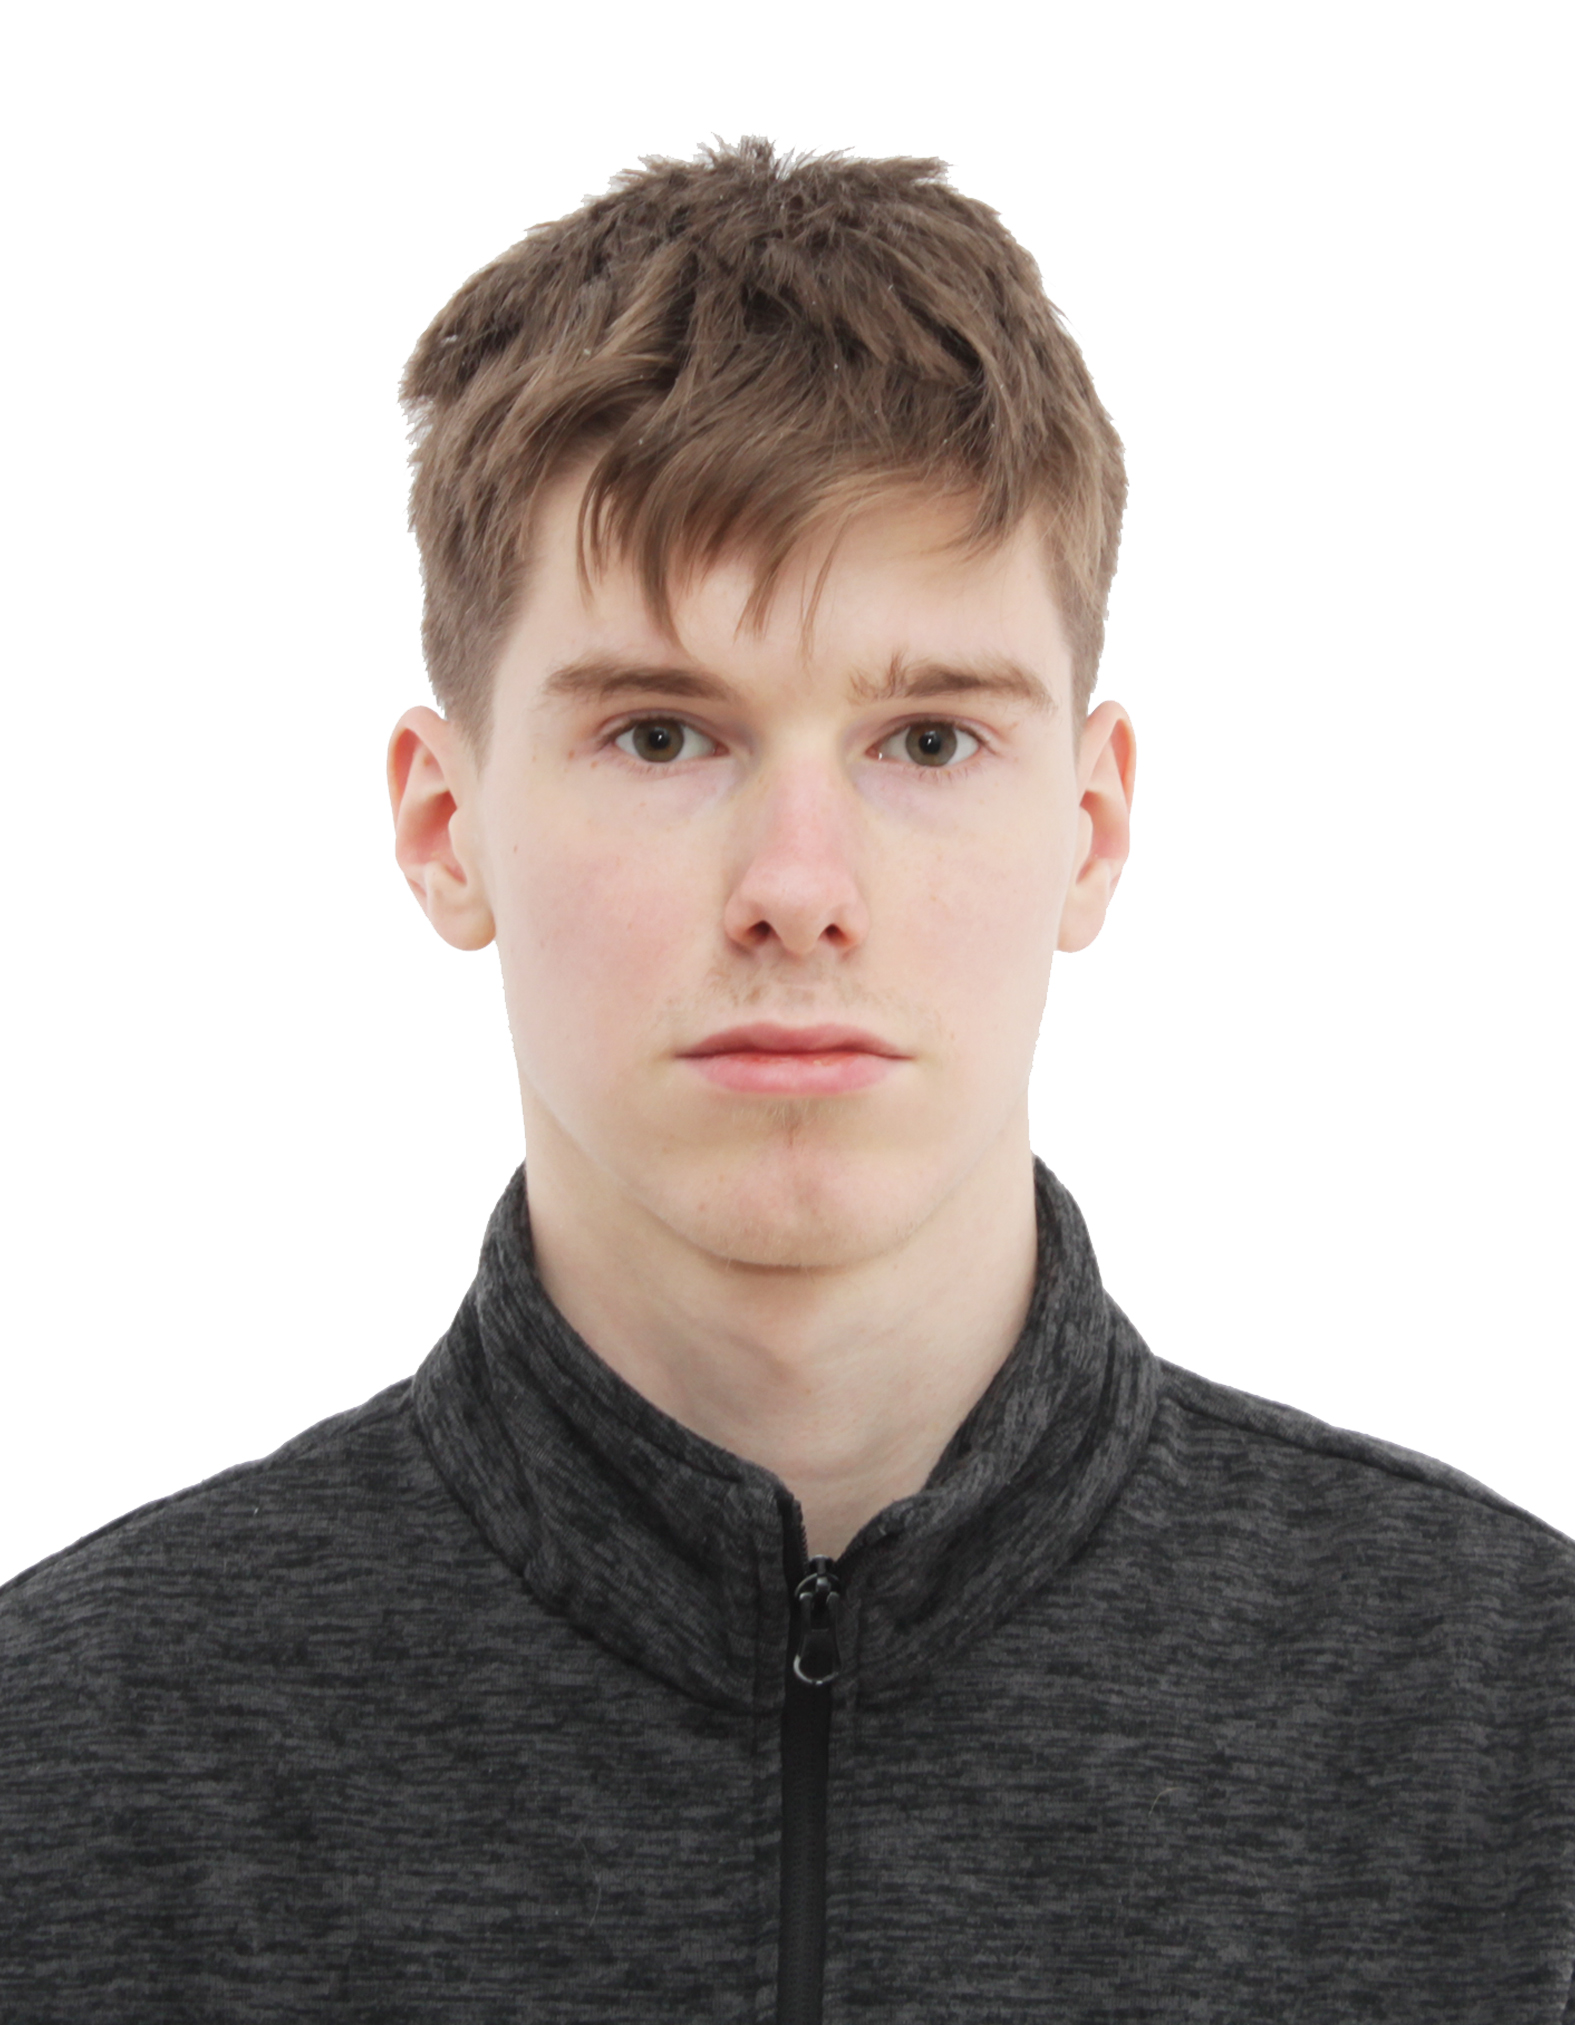
\includegraphics[width=0.6\columnwidth]{photo.jpg}\\[\baselineskip] % Your photo
\small % Smaller font size
Viktor Baldin \\ % Your name
\href{mailto:baldin.va@phystech.edu}{baldin.va@phystech.edu} \\ % Your email address
\href{https://github.com/victorbaldin56}{github.com/victorbaldin56} \\ % Your URL
%\href{https://t.me/victorbaldin_111}{t.me/victorbaldin_111} \\
+7 (916) 582 00 45 \\ % Your phone number
\Sep % Some whitespace
\textbf{Address} \\
34/5 Pervomayskaya St \\ % Address 1
Dolgoprudny, State 141700 \\ % Address 2
Russia \\ % Address 3
\vfill % Whitespace under this block to push it up under the photo
\end{flushright}
}

%----------------------------------------------------------------------------------------

\begin{document}

\userinformation % Print your information in the left column

\framebreak % End of the first column

%----------------------------------------------------------------------------------------
%	HEADING
%----------------------------------------------------------------------------------------

\cvheading{Viktor Baldin} % Large heading - your name

%\cvsubheading{Software Engeneer Job Candidate} % Subheading - your occupation/specialization

%----------------------------------------------------------------------------------------
%	ABOUT ME
%----------------------------------------------------------------------------------------

\aboutme{About Me}{
I am the 1st year MIPT student. Currently I am learning low-level programming because it is interesting
for me to know how actually hardware work. My hobbies are: sports (running), chess, cooking, volunteering.
}

%----------------------------------------------------------------------------------------
%	EDUCATION
%----------------------------------------------------------------------------------------

\CVSection{Education}

%------------------------------------------------

\CVItem{Bachelor, MIPT}{
Bachelor in Applied Mathematics and Physics,
Department of Radio Engeneering and Cybernetics (2023 - present)
}

\CVItem{Educational courses}{
\begin{itemize}
    \item I. R. Dedinsky's "Introduction to Computer System emulation, compiler technologies and
    industrial programming" (2023 - 2024)
\end{itemize}
}

%------------------------------------------------

\Sep % Extra whitespace after the end of a major section


%----------------------------------------------------------------------------------------
%	EXPERIENCE
%----------------------------------------------------------------------------------------

\CVSection{Projects}

%------------------------------------------------

\CVItem{Processor}{
Simple processor emulator with its own stack-based architecture.\\
Link: \url{https://github.com/victorbaldin56/processor}
}

\CVItem{Differenciator}{
A derivative calculator with step-by-step solution. Creates AST for input
mathematical expression and evaluates a derivative by performing operations on AST.\\
Link: \url{https://github.com/victorbaldin56/differenciator}
}

\CVItem{Mandelbrot}{
Mandelbrot fractal
graphical generator built with use of SFML. The main goal of this project was the
research of SIMD instructions to speed up calculations up to several times.\\
Link: \url{https://github.com/victorbaldin56/mandelbrot_fractal}
}

\CVItem{Hash Map}{
Accelerated implementation of hash map.
Educational project to master skills of agressive platform-dependent optimizations.\\
Link: \url{https://github.com/victorbaldin56/hashmap}
}

\CVItem{Binary Translator}{
Continuation of "Processor" project. Translates emulator's bytecode to real x86 opcodes.
Supports dump as NASM assembly or JIT native code execution.\\
Link: \url{https://github.com/victorbaldin56/binary_translator}
}

\Sep % Extra whitespace after the end of a major section

%----------------------------------------------------------------------------------------
%	COMMUNICATION SKILLS
%----------------------------------------------------------------------------------------

\CVSection{Communication skills}

\CVItem{Languages}{
\begin{itemize}
    \item Russian (native)
    \item English (Intermediate)
\end{itemize}
}

\Sep

\CVSection{Software development skills}

%------------------------------------------------

\CVItem{Programming}
{\begin{tabular}{p{0.3\textwidth} p{0.3\textwidth}}
\bluebullet C &  \bluebullet C++ \\
\bluebullet x86 Assembly & \bluebullet Unix Shell\\
\bluebullet Python &  \bluebullet \LaTeX\\
\bluebullet Make &   \bluebullet CMake\\
\end{tabular}}

%------------------------------------------------

\CVItem{Toolchain}
{\begin{tabular}{p{0.3\textwidth} p{0.3\textwidth}}
\bluebullet Profilers (Perf, Valgrind) &  \bluebullet Debuggers (GDB) \\
\bluebullet Assemblers (NASM) &  \bluebullet Disassemblers (objdump)  \\
\bluebullet Version control (Git)
\end{tabular}}

%------------------------------------------------

\Sep % Extra whitespace after the end of a major section

\CVSection{Awards}

\CVItem{Olympiads}{
\begin{itemize}
    \item Phystech Olympiad in Physics, 2nd degree (2023)
    \item Kurchatov Olympiad in Physics, 2nd degree (2023)
    \item Regional Russian Olympiad in Physics, 1st degree (2023)
\end{itemize}
}

\Sep

%----------------------------------------------------------------------------------------
%	NEW PAGE DELIMITER
%	Place this block wherever you would like the content of your CV to go onto the next page
%----------------------------------------------------------------------------------------

%\clearpage % Start a new page
%
%\userinformation % Print your information in the left column
%
%\framebreak % End of the first column
%
%%----------------------------------------------------------------------------------------
%%	AWARDS
%%----------------------------------------------------------------------------------------
%
%\CVSection{Awards}
%
%%------------------------------------------------
%
%\CVItem{2010, \textit{Postgraduate Scholarship}, Cornell University}{Awarded to the top student in their final year of a Bachelors degree.}
%
%%------------------------------------------------
%
%\Sep % Extra whitespace after the end of a major section
%
%%----------------------------------------------------------------------------------------
%%	INTERESTS
%%----------------------------------------------------------------------------------------
%
%\CVSection{Interests}
%
%%------------------------------------------------
%
%\CVItem{Professional}{Data analysis, company profiling, risk analysis, economics, web design, web app creation, software design, marketing}
%
%%------------------------------------------------
%
%\CVItem{Personal}{Piano, chess, cooking, dancing, running}
%
%%------------------------------------------------
%
%\Sep % Extra whitespace after the end of a major section

%----------------------------------------------------------------------------------------

\end{document}
